\documentclass[aps,prl,reprint,superscriptaddress,longbibliography,bibnotes,floatfix]{revtex4-2}
\usepackage{amsmath,amssymb,bm,graphicx}
\usepackage[colorlinks=true,allcolors=blue]{hyperref}
\newcommand{\Tr}{\operatorname{Tr}}
\newcommand{\EC}{\mathrm{EC}}
\newcommand{\CS}{\mathrm{CS}}
\begin{document}
\title{Extensible Causality Does Not Guarantee Pure Quantum Dilations}
\author{Chengxi Li}
\affiliation{Beijing Institute of Petrochemical Technology, Beijing 102617, China}
\affiliation{Beijing National Laboratory for Condensed Matter Physics, Institute of Physics, Chinese Academy of Sciences, Beijing 100190, China}
\author{Hao Zhu}
\affiliation{Beijing Institute of Petrochemical Technology, Beijing 102617, China}
\affiliation{Beijing National Laboratory for Condensed Matter Physics, Institute of Physics, Chinese Academy of Sciences, Beijing 100190, China}
\author{Kai Liu}
\affiliation{Beijing National Laboratory for Condensed Matter Physics, Institute of Physics, Chinese Academy of Sciences, Beijing 100190, China}
\author{Wanzi Sun}
\thanks{Corresponding author. \href{mailto:wzsun@jnxy.edu.cn}{wzsun@jnxy.edu.cn}}
\affiliation{Beijing National Laboratory for Condensed Matter Physics, Institute of Physics, Chinese Academy of Sciences, Beijing 100190, China}
\affiliation{Jining University, Qufu, Shandong 273155, China}
\date{October 10, 2026}
\begin{abstract}
Every ordinary quantum channel admits a reversible explanation on a larger system. We show that extensible causality---causal records for every finite local experiment with arbitrary finite-dimensional shared inputs---does not guarantee such an explanation for a process connecting two laboratories. We construct a full-rank process on four qubit ports that satisfies this requirement yet has no pure process dilation with any finite environment. An operator positivity certificate independent of ancillary dimension establishes causality, while a causal witness and known pure-process structure exclude purification. The separation survives white-noise fractions below $1/11$ and occupies a region of nonzero volume in valid process space. Entanglement-assisted causal tests are therefore insufficient to select processes admitting a reversible quantum dilation.
\end{abstract}
\maketitle

\emph{Introduction.---}Ordinary quantum channels admit a reversible explanation on a larger system~\cite{Stinespring}. Allowing quantum control of laboratory order~\cite{QuantumSwitch,QuantumCausality} raises a physical consistency question: do causal experimental records guarantee that the connection retains such an explanation? Order control offers advantages in channel discrimination~\cite{Discriminate}, computation~\cite{GateOrder}, machine learning~\cite{GongMachineLearning}, and communication~\cite{Communication,NoisyCommunication,PerfectCommunication}, with photonic demonstrations~\cite{Procopio,Rubino,Goswami,WeiExperiment}. Higher-order transformations and quantum networks describe these connections~\cite{Supermaps,CombArchitecture,QuantumNetworks}, whereas process matrices do not assume a global causal order~\cite{OCB}. Purification extends the environmental explanation to these processes~\cite{PurificationAxiom,purif}. Measurement reversibility~\cite{UedaReversibility} and information--disturbance trade-offs~\cite{KimMeasurementTradeoff} distinguish acquired classical information from the preservation of quantum information. Causality tests constrain observable records; purification asks whether the same quantum connection can arise from reversible dynamics.

Yet causal records need not reveal a process's realization. Causal inequalities constrain records~\cite{BranciardCI}; causal witnesses test for a common quantum mixture of ordered processes~\cite{Witness,WitnessGuide}. Feix et al.'s transpose construction~\cite{Feix} produces nonseparable processes with causal models without shared ancillas. With shared entanglement, transposing Bob's operations can also partially transpose the shared state and destroy positivity~\cite{Feix,EC}. Extensible causality requires causal records for every finite experiment with arbitrary finite-dimensional shared inputs~\cite{EC}. A pure dilation must explain one process for all inserted operations~\cite{purif}. Whether extensible causality guarantees separability or purification for two laboratories remained open~\cite{EC,purif}. Pure-process structure~\cite{Yokojima,Cyclic}, spacetime realizations~\cite{TimeDelocalized}, and circuits for extensible causal separability~\cite{Wechs,Wei,Wechs2026} do not resolve this question.

\begin{figure}[!b]
 \centering
 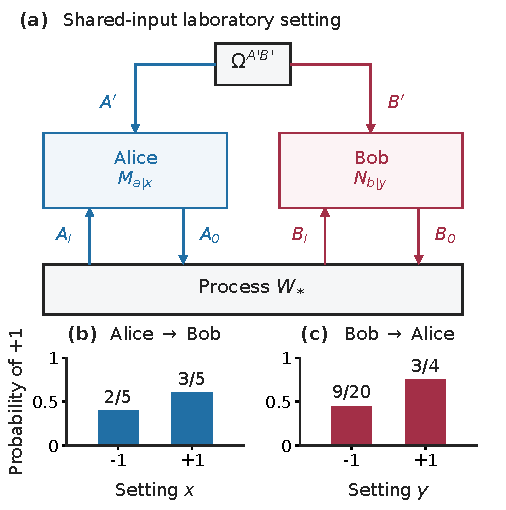
\includegraphics[width=\columnwidth]{laboratory_responses.pdf}
 \caption{Laboratory probes of $W_*$, the chosen counterexample. (a) Alice and Bob receive/return qubit ports marked $I/O$, share ancillary state $\Omega^{A'B'}$, and apply Choi operations $M_{a|x},N_{b|y}$ with settings $x,y$ and outcomes $a,b$. Links identify ports, not a realizing circuit. (b,c) Probabilities of outcome $+1$ for the two protocols in Eq.~\eqref{eq:directional-response}, with settings $\pm1$. Both directions respond; these experiments alone do not certify nonseparability.}
 \label{fig:laboratories}
\end{figure}

Here we answer both questions negatively. Our full-rank process on four qubit ports inherits its ordinary causal model from that transpose construction. Our new dimension-independent positivity certificate proves causality for arbitrary finite shared inputs and all finite local experiments. Local preparations and measurements expose both directions of influence. A witness excludes any common quantum mixture of orders; known pure-process structure~\cite{Yokojima,Cyclic} rules out every finite pure dilation. The separation survives white noise and fills a nonzero-volume region. Purification thus requires more than entanglement-assisted causal tests.

\emph{Laboratory setting.---}Shared quantum resources and local operations underlie atomic-ensemble communication~\cite{DuanQuantumNetworks}, proposals for high-dimensional photonic gates~\cite{XiaPhotonicGate}, and teleportation-based quantum interfaces~\cite{ZhangTeleportation}. In our setting, each laboratory receives a quantum input and returns a quantum output. Alice chooses a setting $x$, records $a$, and applies a completely positive instrument with Choi matrices $M_{a|x}$. Bob chooses $y$, records $b$, and uses $N_{b|y}$. The ports $A_I,A_O,B_I,B_O$ belong to Alice and Bob, respectively; subscripts $I,O$ denote input and output. With a shared input state $\Omega^{A'B'}$ on their local ancillary spaces $A',B'$, the process matrix $W$ gives
\begin{equation}
 p(a,b|x,y)=\Tr[(W\otimes\Omega^{A'B'})
                    (M_{a|x}\otimes N_{b|y})],
 \label{eq:born-main}
\end{equation}
where the left side is the joint outcome probability conditional on the settings; $\Tr$ and $\otimes$ denote trace and tensor product. Summing each instrument over outcomes gives a trace-preserving channel. We use the full-transpose Choi convention in the Supplemental Material~\cite{SM}. Process constraints ensure normalized, nonnegative probabilities without assuming a circuit~\cite{OCB}.

A causal explanation of the records has the form
\begin{equation}
 p=q\,p^{A\prec B}+(1-q)\,p^{B\prec A},
 \label{eq:causal-model}
\end{equation}
where $p$ is the complete probability table, the superscripted terms are normalized ordered tables, and $q$ is the setting-independent Alice-first probability. The notation $A\prec B$ means Alice's marginal is independent of $y$, while Bob may respond to $x$; $B\prec A$ reverses this condition. Extensible causality (EC) requires such a model for every finite shared ancillary state and every finite experiment, with all settings and outcomes~\cite{EC}. The model may depend on the experiment. Causal separability (CS) requires one positive mixture of ordered \emph{processes} reproducing all instruments.

\emph{Competing directions of influence.---}All four original ports are qubits. Let $\sigma_x,\sigma_y,\sigma_z$ denote the Pauli matrices. A superscript identifies the port on which a matrix acts; omitted ports carry the identity. Products on distinct ports denote tensor products in the order $A_I,A_O,B_I,B_O$, and $I$ is the identity on all four ports. Our example is
\begin{align}
 W_* =\frac14\Bigl[&I+\frac15\sigma_z^{A_I}
 +\frac3{10}\sigma_z^{A_I}\sigma_x^{B_I}\sigma_z^{B_O}\notag\\
 &+\frac15\sum_{k=x,y,z}\sigma_k^{A_O}\sigma_k^{B_I}\Bigr],
 \label{eq:process}
\end{align}
where $k$ labels the three Pauli axes, and the asterisk labels this counterexample. It has trace four, obeys process normalization, and has minimum eigenvalue $1/40$, ensuring strict positivity.

The term $\sigma_z^{A_I}$ biases Alice's input. The three $A_O$--$B_I$ couplings transmit Alice's preparation to Bob's measurement; $\sigma_z^{A_I}\sigma_x^{B_I}\sigma_z^{B_O}$ carries reverse dependence through Alice's input and Bob's ports. Commutation with $\sigma_z^{A_I}$ and $\sigma_z^{B_O}$ makes these two ports classical labels in their respective bases. The other ports retain noncommuting Pauli correlations.

Two protocols expose these dependences (Fig.~\ref{fig:laboratories}). First, Alice discards her input and prepares a $\sigma_x^{A_O}$ eigenstate with eigenvalue $x=\pm1$. Bob measures $\sigma_x^{B_I}$, records $b=\pm1$, and returns a maximally mixed output. Second, Bob measures $\sigma_x^{B_I}$, obtains $r=\pm1$, and prepares a $\sigma_z^{B_O}$ eigenstate with eigenvalue $yr$; $y=\pm1$ is his setting. Alice measures $\sigma_z^{A_I}$, records $s=\pm1$, and returns a maximally mixed output. The Born rule gives
\begin{equation}
 \langle b\rangle_x=\frac{x}{5},\qquad
 \langle s\rangle_y=\frac15+\frac{3y}{10},
 \label{eq:directional-response}
\end{equation}
where angle brackets denote outcome averages conditional on the subscripted setting. Switching the settings changes the receivers' $+1$ probabilities by $1/5$ and $3/10$. A random mixture of orders can also display both responses in these separate experiments. The stronger question is whether \emph{one quantum mixture} accounts for all operations on this process.

\begin{figure}[!t]
 \centering
 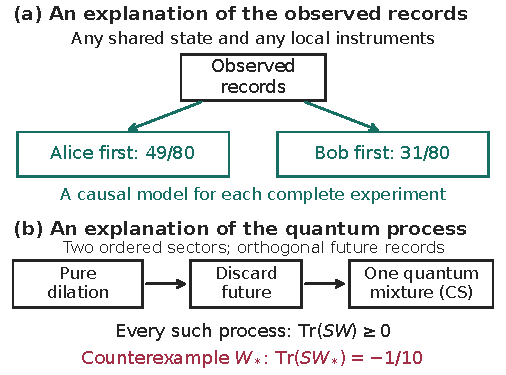
\includegraphics[width=\columnwidth]{causal_purification.pdf}
 \caption{Different demands on records and processes. (a) Every finite shared-input experiment on $W_*$ admits Alice-first/Bob-first records with weights $49/80$ and $31/80$. Branch records may depend on the experiment. (b) In our bipartite setting, discarding the orthogonal future records of a pure dilation yields one positive mixture of ordered processes: causal separability (CS). The causal witness $S$ has nonnegative trace pairing on this set, but is negative on the counterexample; Tr denotes trace. The diagram summarizes the proof.}
 \label{fig:separation}
\end{figure}

\emph{Why a pure dilation is excluded.---}A pure dilation adds a global past and future, prepares a fixed pure past state, and discards the future~\cite{purif}; their dimensions are arbitrary finite. Our original process has no global input or output. In this bipartite setting, a reversible process splits into two ordered sectors with orthogonal future records~\cite{Yokojima,Cyclic}. Discarding these records leaves a positive mixture of orders (Fig.~\ref{fig:separation}). Conversely, retaining its environments and order record dilates such a mixture. Hence
\begin{equation}
 \mathrm{Purifiable}=\CS\subseteq\EC,
 \label{eq:known}
\end{equation}
where the labels denote process sets. The argument allows arbitrary finite past and future dimensions, without a rank-based environment bound.

For $W_*$, a causal witness $S$ made from a singlet projector on $A_OB_I$ and Pauli terms satisfies $\Tr(SW)\ge0$ for every CS process, whereas
\begin{equation}
 \Tr(SW_*)=-\frac1{10}.
 \label{eq:witness-value}
\end{equation}
The Supplemental Material proves witness positivity on both ordered cones~\cite{SM}. Trusted process tomography reconstructs the Pauli coefficients of $W$ from measured probabilities and knowledge of the calibrated local operations~\cite{Trusted,Network}. The negative value excludes the common quantum mixture and hence every finite pure dilation. Standard deterministic quantum circuits with quantum control of causal order (QC-QC) have a pure extension upon retaining their internal environments~\cite{QCQC}, excluding their realization of $W_*$ here.

\emph{Causality survives arbitrary entangled probes.---}Our result covers all local instruments, arbitrary finite shared entangled inputs, and all finite settings and outcomes. A single order weight $q=\frac{49}{80}$ works throughout; the causal explanation in Fig.~\ref{fig:separation}(a) follows from an operator identity.

Reporting the two classical port labels refines outcomes; discarding them recovers the original probabilities. Each joint outcome's probability must be split between the two orders. We prescribe nonnegative first-party contributions $g_a(x)$ and $h_b(y)$ of total weights $q$ and $1-q$, respectively. Each depends only on its own setting and remains unchanged across the other laboratory's choices.

The joint probabilities can be assigned to these branches precisely when every pair of accepted outcome groups $\mathcal A,\mathcal B$ obeys
\begin{equation}
 p(\mathcal A,\mathcal B|x,y)
 \le g(\mathcal A|x)+h(\mathcal B|y),
 \label{eq:hall}
\end{equation}
where both sides sum over the indicated outcome groups. Accepting both groups cannot exceed the prescribed first-party contributions. A capacitated transportation theorem converts these inequalities, including empty and full groups, into the complete causal model~\cite{SM}.

For a pure shared input with Bob marginal $\rho$, where $\Tr\rho=1$, let $\tau_s$ be Bob's subnormalized conditional marginal for the accepted Alice group in input-flag sector $s=\pm1$. Let $E$ be Bob's accepted effect on $B_IB'$. Explicitly,
\begin{equation}
\begin{split}
 g(\mathcal A|x)&=\sum_{s=\pm1}\frac{245+48s}{800}\Tr\tau_s,\\
 h(\mathcal B|y)&=\frac{31}{160}\Tr[(I_{B_I}\otimes\rho)E],\\
 g+h-p&=\frac{\langle\Psi|\mathcal Q|\Psi\rangle}{4\,000\,000}\ge0,
\end{split}
\label{eq:positive-gap}
\end{equation}
where $I_{B_I}$ is the input-qubit identity, $g,h,p$ in the last line abbreviate the three quantities in Eq.~\eqref{eq:hall}, and $|\Psi\rangle$ is the normalized shared input embedded in enlarged local ancillary spaces. The positive semidefinite operator $\mathcal Q$ is the sum of fifteen positive operator contractions printed in the Supplemental Material~\cite{SM}. Its integer coefficient matrices have size at most four; the operators they weight may act on ancillary spaces of any finite dimension. The contributions have the required total weights $q$ and $1-q$.

Retaining Alice's Kraus environment and applying a Naimark dilation to Bob's effects preserve the probabilities and these contributions for general instruments, including complex amplitudes and multiple Kraus branches. The identity uses only the positive remainder for Alice's rejected event, Bob's projector relations, and commutation between laboratories, so it holds in every finite ancillary dimension. Mixed shared states follow by convexity with the same $q$. No such experiment can therefore violate a causal inequality; optimization only discovers the exact certificate.

\begin{figure}[!t]
 \centering
 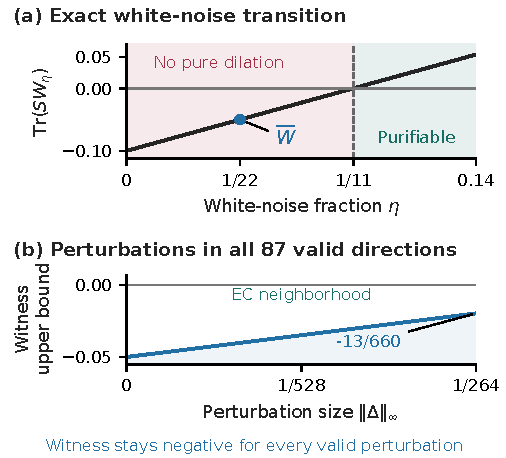
\includegraphics[width=\columnwidth]{counterexample_noise.pdf}
 \caption{Separation survives noise and general perturbations. (a) Exact trace pairing of witness $S$ with the noisy process $W_\eta$; $\eta$ is the uniform replacement probability. The whole noise line is EC. Shading meets at the exact pure-dilation threshold $1/11$; this plot enlarges its vicinity. The blue point is $\overline W=W_{1/22}$. (b) Upper bound $-1/20+8\|\Delta\|_\infty$ for that witness about $\overline W$; $\Delta$ is a valid Hermitian trace-zero perturbation and its norm is its largest absolute eigenvalue. Every such direction remains EC with negative witness within this sufficient radius, which is not an optimal boundary.}
 \label{fig:noise}
\end{figure}

\emph{Stability under noise and general perturbations.---}The separation has a finite noise tolerance. Let the uniform process $I/4$ replace $W_*$ with probability $\eta$:
\begin{equation}
 W_\eta=(1-\eta)W_*+\eta I/4,\qquad0\le\eta\le1.
 \label{eq:noise}
\end{equation}
Replacement erases the directional responses with probability $\eta$. Convexity preserves EC along the whole line. The witness becomes $(11\eta-1)/10$, excluding pure dilation below $1/11$, or approximately $9.1\%$ white noise. An explicit positive ordered decomposition at the threshold~\cite{SM} gives
\begin{align}
 &W_\eta\in\EC\quad\forall\eta,\notag\\
 &W_\eta\in\mathrm{Purifiable}\Longleftrightarrow
 W_\eta\in\CS\Longleftrightarrow\eta\ge\frac1{11},
 \label{eq:noise-classification}
\end{align}

where membership refers to process sets, the double arrows mean ``if and only if,'' and ``for all'' covers the full noise interval. Noise restores a pure explanation while records remain causal on both sides [Fig.~\ref{fig:noise}(a)].

General perturbations may also break the Pauli pattern. With $W_0=I/4$ the uniform process, define the neighborhood center
\begin{equation}
 \overline W=\frac{21}{22}W_*+\frac1{22}W_0.
 \label{eq:robust-center}
\end{equation}
For every Hermitian, trace-zero perturbation $\Delta$ in the valid process linear subspace,
\begin{equation}
 \|\Delta\|_\infty\le\frac1{264}
 \ \Longrightarrow\ 
 \overline W+\Delta\in\EC\setminus\CS,
 \label{eq:robust-ball}
\end{equation}
where the norm is the largest absolute perturbation eigenvalue; the set difference means EC but not CS. For trace four, the bound covers all 87 valid directions, including broken classical-label symmetries. Mixing with a CS neighborhood of the uniform process retains EC and a strictly negative witness~\cite{SM} [Fig.~\ref{fig:noise}(b)]. The sufficient radius is neither an optimal boundary nor a laboratory-error percentage; it does not establish that $W_*$ itself is interior to EC.

\emph{Discussion.---}Requiring causal records in every entanglement-assisted experiment is an insufficient criterion for selecting reversible higher-order dynamics. A causal model may adapt to each experiment; a pure dilation must explain the same process for all inserted operations. In our example, every causal-inequality test yields compatible records, even with arbitrary finite shared inputs. Trusted tomography adds calibrated knowledge of the local quantum operations: it reconstructs one process operator across experiments, and the negative witness value then excludes every finite pure-process dilation. Thus the absence of a causal-inequality violation cannot certify such a realization. Information preservation under monitoring is also studied through the competition between unitary scrambling and measurements~\cite{QiMonitoredQEC}. Environmental descriptions of cavity decay~\cite{GarrawayPseudomode}, entanglement loss~\cite{YuSuddenDeath}, and dissipative excitation transfer~\cite{PuOpenSystem}, as well as effective non-Hermitian many-body models~\cite{Li2024NonHermitian}, specify dynamics for a given system. The present obstruction concerns the higher-order connection that must accommodate every local operation. The result concerns two laboratories with qubit ports and no original global past or future. Its QC-QC consequence applies to standard deterministic circuits using each operation once~\cite{QCQC}; postselected simulations, other realization frameworks, and multiple-use composition lie outside this statement.

In summary, we establish a robust separation between extensible causality and finite pure-process realizability. Our full-rank process remains causal for arbitrary finite shared inputs and every finite local experiment, yet has no finite pure dilation. Noise tolerance and a nonzero-volume neighborhood show that the gap is stable. Reversible realization therefore requires a consistency criterion beyond entanglement-assisted causal tests.

\emph{Data availability.---}The exact certificates and portable verification code are publicly available in the \href{https://github.com/phycxli/Extensible-Causality-Does-Not-Guarantee-Pure-Quantum-Dilations}{GitHub repository} and in the accompanying supplemental files. They check the process, witness, laboratory responses, and stability without optimization.

\emph{Acknowledgments.---}We thank Dr. Tianyu Xie of Xiamen University for providing computational resources and Dr. Tie-Fu Zhang for helpful discussions. This work is supported by the Zhiyuan Science Foundation of BIPT (No. 2026210).

\begin{thebibliography}{99}
\bibitem{Stinespring} W. F. Stinespring, Positive functions on $C^*$-algebras, \href{https://doi.org/10.1090/S0002-9939-1955-0069403-4}{Proc. Am. Math. Soc. \textbf{6}, 211 (1955)}.
\bibitem{QuantumSwitch} G. Chiribella, G. M. D'Ariano, P. Perinotti, and B. Valiron, Quantum computations without definite causal structure, \href{https://doi.org/10.1103/PhysRevA.88.022318}{Phys. Rev. A \textbf{88}, 022318 (2013)}.
\bibitem{QuantumCausality} C. Brukner, Quantum causality, \href{https://doi.org/10.1038/nphys2930}{Nat. Phys. \textbf{10}, 259 (2014)}.
\bibitem{Discriminate} G. Chiribella, Perfect discrimination of no-signalling channels via quantum superposition of causal structures, \href{https://doi.org/10.1103/PhysRevA.86.040301}{Phys. Rev. A \textbf{86}, 040301(R) (2012)}.
\bibitem{GateOrder} M. Ara\'{u}jo, F. Costa, and C. Brukner, Computational Advantage from Quantum-Controlled Ordering of Gates, \href{https://doi.org/10.1103/PhysRevLett.113.250402}{Phys. Rev. Lett. \textbf{113}, 250402 (2014)}.
\bibitem{GongMachineLearning} N. Ma, P. Z. Zhao, and J. Gong, Quantum machine learning with indefinite causal order, \href{https://doi.org/10.1103/PhysRevA.110.052406}{Phys. Rev. A \textbf{110}, 052406 (2024)}.
\bibitem{Communication} P. A. Gu\'{e}rin, A. Feix, M. Ara\'{u}jo, and C. Brukner, Exponential Communication Complexity Advantage from Quantum Superposition of the Direction of Communication, \href{https://doi.org/10.1103/PhysRevLett.117.100502}{Phys. Rev. Lett. \textbf{117}, 100502 (2016)}.
\bibitem{NoisyCommunication} D. Ebler, S. Salek, and G. Chiribella, Enhanced Communication with the Assistance of Indefinite Causal Order, \href{https://doi.org/10.1103/PhysRevLett.120.120502}{Phys. Rev. Lett. \textbf{120}, 120502 (2018)}.
\bibitem{PerfectCommunication} G. Chiribella \emph{et al.}, Indefinite causal order enables perfect quantum communication with zero capacity channels, \href{https://doi.org/10.1088/1367-2630/abe7a0}{New J. Phys. \textbf{23}, 033039 (2021)}.
\bibitem{Procopio} L. M. Procopio \emph{et al.}, Experimental superposition of orders of quantum gates, \href{https://doi.org/10.1038/ncomms8913}{Nat. Commun. \textbf{6}, 7913 (2015)}.
\bibitem{Rubino} G. Rubino \emph{et al.}, Experimental verification of an indefinite causal order, \href{https://doi.org/10.1126/sciadv.1602589}{Sci. Adv. \textbf{3}, e1602589 (2017)}.
\bibitem{Goswami} K. Goswami \emph{et al.}, Indefinite Causal Order in a Quantum Switch, \href{https://doi.org/10.1103/PhysRevLett.121.090503}{Phys. Rev. Lett. \textbf{121}, 090503 (2018)}.
\bibitem{WeiExperiment} K. Wei \emph{et al.}, Experimental Quantum Switching for Exponentially Superior Quantum Communication Complexity, \href{https://doi.org/10.1103/PhysRevLett.122.120504}{Phys. Rev. Lett. \textbf{122}, 120504 (2019)}.
\bibitem{Supermaps} G. Chiribella, G. M. D'Ariano, and P. Perinotti, Transforming quantum operations: Quantum supermaps, \href{https://doi.org/10.1209/0295-5075/83/30004}{Europhys. Lett. \textbf{83}, 30004 (2008)}.
\bibitem{CombArchitecture} G. Chiribella, G. M. D'Ariano, and P. Perinotti, Quantum Circuit Architecture, \href{https://doi.org/10.1103/PhysRevLett.101.060401}{Phys. Rev. Lett. \textbf{101}, 060401 (2008)}.
\bibitem{QuantumNetworks} G. Chiribella, G. M. D'Ariano, and P. Perinotti, Theoretical framework for quantum networks, \href{https://doi.org/10.1103/PhysRevA.80.022339}{Phys. Rev. A \textbf{80}, 022339 (2009)}.
\bibitem{OCB} O. Oreshkov, F. Costa, and C. Brukner, Quantum correlations with no causal order, \href{https://doi.org/10.1038/ncomms2076}{Nat. Commun. \textbf{3}, 1092 (2012)}.
\bibitem{PurificationAxiom} G. Chiribella, G. M. D'Ariano, and P. Perinotti, Probabilistic theories with purification, \href{https://doi.org/10.1103/PhysRevA.81.062348}{Phys. Rev. A \textbf{81}, 062348 (2010)}.
\bibitem{purif} M. Ara\'{u}jo, A. Feix, M. Navascu\'{e}s, and C. Brukner, A purification postulate for quantum mechanics with indefinite causal order, \href{https://doi.org/10.22331/q-2017-04-26-10}{Quantum \textbf{1}, 10 (2017)}.
\bibitem{UedaReversibility} M. Ueda and M. Kitagawa, Reversibility in quantum measurement processes, \href{https://doi.org/10.1103/PhysRevLett.68.3424}{Phys. Rev. Lett. \textbf{68}, 3424 (1992)}.
\bibitem{KimMeasurementTradeoff} S. Hong, Y.-S. Kim, Y.-W. Cho, J. Kim, S.-W. Lee, and H.-T. Lim, Demonstration of Complete Information Trade-Off in Quantum Measurement, \href{https://doi.org/10.1103/PhysRevLett.128.050401}{Phys. Rev. Lett. \textbf{128}, 050401 (2022)}.
\bibitem{BranciardCI} C. Branciard, M. Ara\'{u}jo, A. Feix, F. Costa, and C. Brukner, The simplest causal inequalities and their violation, \href{https://doi.org/10.1088/1367-2630/18/1/013008}{New J. Phys. \textbf{18}, 013008 (2016)}.
\bibitem{Witness} M. Ara\'{u}jo \emph{et al.}, Witnessing causal nonseparability, \href{https://doi.org/10.1088/1367-2630/17/10/102001}{New J. Phys. \textbf{17}, 102001 (2015)}.
\bibitem{WitnessGuide} C. Branciard, Witnesses of causal nonseparability: an introduction and a few case studies, \href{https://doi.org/10.1038/srep26018}{Sci. Rep. \textbf{6}, 26018 (2016)}.
\bibitem{Feix} A. Feix, M. Ara\'{u}jo, and C. Brukner, Causally nonseparable processes admitting a causal model, \href{https://doi.org/10.1088/1367-2630/18/8/083040}{New J. Phys. \textbf{18}, 083040 (2016)}.
\bibitem{EC} O. Oreshkov and C. Giarmatzi, Causal and causally separable processes, \href{https://doi.org/10.1088/1367-2630/18/9/093020}{New J. Phys. \textbf{18}, 093020 (2016)}.
\bibitem{Yokojima} W. Yokojima, M. T. Quintino, A. Soeda, and M. Murao, Consequences of preserving reversibility in quantum superchannels, \href{https://doi.org/10.22331/q-2021-04-26-441}{Quantum \textbf{5}, 441 (2021)}.
\bibitem{Cyclic} J. Barrett, R. Lorenz, and O. Oreshkov, Cyclic quantum causal models, \href{https://doi.org/10.1038/s41467-020-20456-x}{Nat. Commun. \textbf{12}, 885 (2021)}.
\bibitem{TimeDelocalized} O. Oreshkov, Time-delocalized quantum subsystems and operations: on the existence of processes with indefinite causal structure in quantum mechanics, \href{https://doi.org/10.22331/q-2019-12-02-206}{Quantum \textbf{3}, 206 (2019)}.
\bibitem{Wechs} J. Wechs, A. A. Abbott, and C. Branciard, On the definition and characterisation of multipartite causal (non)separability, \href{https://doi.org/10.1088/1367-2630/aaf352}{New J. Phys. \textbf{21}, 013027 (2019)}.
\bibitem{Wei} W. Wei and S. Pang, Extensibly Causally Separable Processes Admit Realizations as Quantum Circuits with Classical Control of Causal Order, arXiv:2609.18559v1 (2026).
\bibitem{Wechs2026} J. Wechs, A. A. Abbott, and C. Branciard, All causally separable quantum processes are quantum circuits with classical control of causal order, arXiv:2609.20774v1 (2026).
\bibitem{DuanQuantumNetworks} L.-M. Duan, M. D. Lukin, J. I. Cirac, and P. Zoller, Long-distance quantum communication with atomic ensembles and linear optics, \href{https://doi.org/10.1038/35106500}{Nature \textbf{414}, 413 (2001)}.
\bibitem{XiaPhotonicGate} M. Chen, J.-S. Tang, M. Cai, Y. Lu, F. Nori, and K. Xia, High-dimensional two-photon quantum controlled phase-flip gate, \href{https://doi.org/10.1103/PhysRevResearch.6.033004}{Phys. Rev. Research \textbf{6}, 033004 (2024)}.
\bibitem{ZhangTeleportation} X.-W. Luo, C. Zhang, I. Novikova, C. Qian, and S. Du, Wavelength conversion for single-photon polarization qubits through continuous-variable quantum teleportation, \href{https://doi.org/10.1103/PhysRevA.105.052444}{Phys. Rev. A \textbf{105}, 052444 (2022)}.
\bibitem{SM} See Supplemental Material for process physicality, the general Born reduction, the transportation theorem, all rational SOS matrices, and independent verification commands.
\bibitem{Trusted} H. Dourdent \emph{et al.}, Semi-Device-Independent Certification of Causal Nonseparability with Trusted Quantum Inputs, \href{https://doi.org/10.1103/PhysRevLett.129.090402}{Phys. Rev. Lett. \textbf{129}, 090402 (2022)}.
\bibitem{Network} H. Dourdent \emph{et al.}, Network-Device-Independent Certification of Causal Nonseparability, \href{https://doi.org/10.22331/q-2024-10-30-1514}{Quantum \textbf{8}, 1514 (2024)}.
\bibitem{QCQC} J. Wechs, H. Dourdent, A. A. Abbott, and C. Branciard, Quantum circuits with classical versus quantum control of causal order, \href{https://doi.org/10.1103/PRXQuantum.2.030335}{PRX Quantum \textbf{2}, 030335 (2021)}.
\bibitem{QiMonitoredQEC} S. Choi, Y. Bao, X.-L. Qi, and E. Altman, Quantum Error Correction in Scrambling Dynamics and Measurement-Induced Phase Transition, \href{https://doi.org/10.1103/PhysRevLett.125.030505}{Phys. Rev. Lett. \textbf{125}, 030505 (2020)}.
\bibitem{GarrawayPseudomode} B. M. Garraway, Nonperturbative decay of an atomic system in a cavity, \href{https://doi.org/10.1103/PhysRevA.55.2290}{Phys. Rev. A \textbf{55}, 2290 (1997)}.
\bibitem{YuSuddenDeath} T. Yu and J. H. Eberly, Sudden Death of Entanglement, \href{https://doi.org/10.1126/science.1167343}{Science \textbf{323}, 598 (2009)}.
\bibitem{PuOpenSystem} D. Fallas Padilla, V. So, A. Menon, R. Zhuravel, H. Pu, and G. Pagano, Delocalized Excitation Transfer in Open Quantum Systems with Long-Range Interactions, \href{https://doi.org/10.1103/bxwl-sbsn}{PRX Quantum \textbf{6}, 040301 (2025)}.
\bibitem{Li2024NonHermitian} C. Li, Y. Wu, and W.-M. Liu, Non-Hermitian superfluid--Mott-insulator transition in the one-dimensional zigzag bosonic chains, \href{https://doi.org/10.1103/PhysRevB.109.214306}{Phys. Rev. B \textbf{109}, 214306 (2024)}.
\end{thebibliography}
\end{document}
